\section{The Measurement Platform in Detail}\label{app:platform}

\paragraph{Live fleet plane}
The public-facing deployment is a three-arm field study behind one SSH face:
arm~A serves a stock shell emulator with no generative backend, arm~B a
bare-LLM persona baseline, and arm~C the full verified deception
pipeline, one arm per host, which isolates the arms from each other while
confounding arm identity with host/IP effects---a design that separates
deployment lanes, not one that identifies endpoint effects apart from
them.
Arm~C's deception loop is a producer--reviewer pipeline (behavioral
classification, threat-intelligence retrieval, response generation) wrapped
in a fail-closed verification chain: a turn whose fiction-consistency or
evasion check fails is never served. Sessions run in sandboxes under
append-only JSONL logging behind an authenticated mTLS transport, and
honeytokens arm the canary gates.

\begin{figure}[t]
\centering
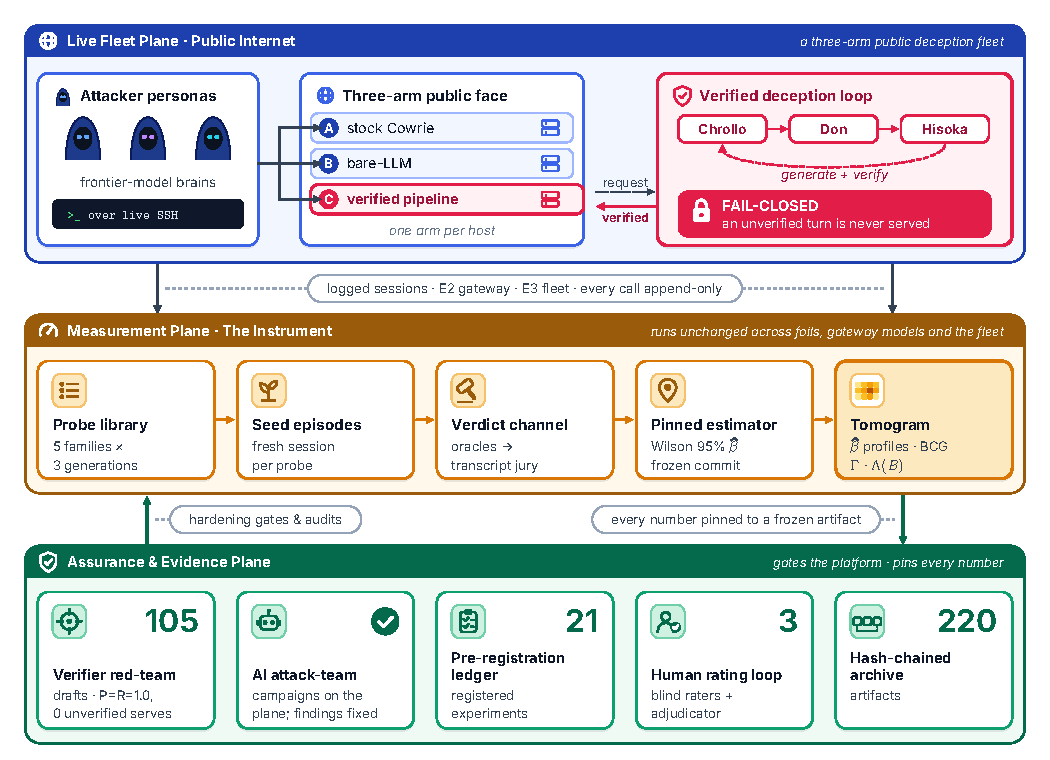
\includegraphics[width=\columnwidth]{anthro/fig3_platform.pdf}
\Description{A layered block diagram of the belief-tomography platform: a
three-arm public deception fleet behind one SSH face with a fail-closed
verified loop, the instrument layer (probe library, verdicts, frozen
estimator) running unchanged across foils, gateway models, and the fleet,
and an assurance--evidence layer gating the platform and pinning reported
numbers.}
\caption{The belief-tomography platform: a three-arm public deception fleet
whose verified loop fails closed; the instrument of
Section~\ref{sec:library} running unchanged across foils, gateway models,
and the fleet; and the assurance--evidence layer that gates the platform and
pins every reported number.}
\label{fig:platform}
\end{figure}

\paragraph{Adversarial assurance and evidence plane}
The platform's own defenses are measured like everything else. Labeled
adversarial drafts run through the real fiction-consistency verifier, and
in the retained serve logs every delivered record carries a passed
verifier check (no unverified serves); the earlier draft's specific
``105 cases, precision 1.0/recall 1.0'' calibration figure is withdrawn
as not reconstructible from the deposit. The
model-visible leakage audit covers the four completed field panels
(1{,}200 sessions, 1{,}600 turns; Section~\ref{sec:e2}); and every number
in this paper is
pinned by the claims--evidence ledger and its SHA-256 artifact manifest
(\texttt{CLAIMS\_EVIDENCE\_LEDGER.md} and
\texttt{ARTIFACT\_MANIFEST.sha256}, Data Availability), which hash the
registration and result artifacts as frozen---including the post-hoc
registration-file edits disclosed in Section~\ref{sec:limits}.
The decision layers and their gate studies (the Laya strategy selector,
held out of the default deployment; the JEV evidence judge, advisory-only)
and the claims--evidence ledger with its
manifest ship with the artifact package; the manifest's SHA-256
enumeration is the claim-to-artifact inventory (an earlier draft vouched a
separate ``codebase inventory,'' which has no on-disk artifact and is
withdrawn in favor of the manifest).

